% Data understanding (frames and speaker notes by Lam, ported to the HUST theme).
% Figures: slide/figures/{monthly_revenue_customers,repurchase_gap,rfm_segment_share}.png, taken from
% Lam's final Data Understanding deck (5 Nov 2026);
% numbers: notebooks/01_data_understanding.ipynb and notebooks/02_customer_segments.ipynb.
\section{Data Understanding}

% Gray field card for the data overview: {title}{fields}{use}
\newcommand{\fieldcard}[3]{%
  \infocard{\dimexpr.5\linewidth-17pt\relax}{1.74cm}{%
    {\large\bfseries\color{hustred}#1}\\[1pt]
    {\footnotesize\bfseries #2}\\[1pt]
    {\scriptsize\color{inkgray}#3}}%
}

\begin{frame}{Data overview}{Online Retail II: 1.07M transaction lines from 5,942 customers, Dec 2009 -- Dec 2011}
  \vspace*{-0.27cm}
  \begin{columns}[T]
    \column{.34\textwidth}
    \infocard[hustred]{\dimexpr\linewidth-14pt\relax}{5.15cm}{\color{white}%
      {\scriptsize\bfseries\color{hustsubyellow}DATA SOURCE}\\[1pt]
      {\LARGE\bfseries Online Retail II}\\[2pt]
      {\small Transactions of an online retailer, Dec 2009 -- Dec 2011}\par
      \vspace{0.5cm}
      {\color{hustsubyellow}\rule{\linewidth}{0.8pt}}\par
      \vspace{3pt}
      \begin{tabular}{@{}p{0.58\linewidth}@{}p{0.40\linewidth}@{}}
        {\bfseries\Large 1,067,371} & {\bfseries\Large 53,628}\\[-4pt]
        {\scriptsize transaction lines} & {\scriptsize invoices}\\[2pt]
        {\bfseries\Large 5,942} & {\bfseries\Large \pounds19.3M}\\[-4pt]
        {\scriptsize customers} & {\scriptsize total revenue}\\[2pt]
        {\bfseries\Large 43} & {\bfseries\Large 8}\\[-4pt]
        {\scriptsize countries, UK 91.9\%} & {\scriptsize fields}
      \end{tabular}}
    \column{.64\textwidth}
    \fieldcard{Customer}{Customer ID, Country}{Identify customers and support segmentation.}\hfill
    \fieldcard{Transactions}{Invoice, InvoiceDate, Quantity, Price}{Build order history and purchase metrics.}\par
    \vspace{3pt}
    \fieldcard{Products}{StockCode, Description}{Measure product diversity and purchase patterns.}\hfill
    \fieldcard{Time and labels}{Customer ID, InvoiceDate, valid purchases}{Create observation windows and define churn in the prediction horizon.}\par
    \vspace{3pt}
    \notebox{\dimexpr\linewidth-14pt\relax}{\footnotesize\textbf{Limitation}: no campaign or marketing-cost fields, so campaign ROI cannot be measured directly.}
  \end{columns}
  % Speaker notes (Lam): Our starting question is simple: with a limited retention budget,
  % which customers should we keep, and when should we act? All we have is two years of
  % transactions from an online retailer: about a million lines and 5,900 customers. There
  % are no contracts and no marketing costs, so both value and churn have to be inferred
  % from how people buy. (About 20 seconds)
\end{frame}

\begin{frame}{Revenue and customers}{Revenue is seasonal, and repeat customers carry it}
  \vspace*{-0.15cm}
  \begin{columns}[T]
    \column{.46\textwidth}
    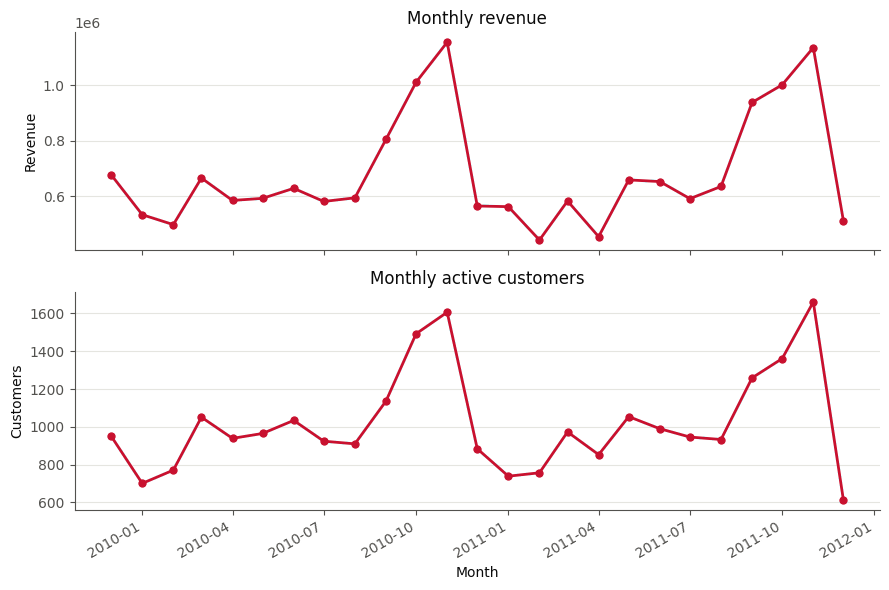
\includegraphics[width=\linewidth]{figures/monthly_revenue_customers.png}
    \column{.52\textwidth}
    \infobox{\dimexpr\linewidth-14pt\relax}{%
      {\large\bfseries\color{hustred}$\sim$1,040 customers/month}\\[3pt]
      {\small\color{inkgray}Median revenue $\approx$ \pounds595K/month (\pounds442K -- \pounds1.16M).}}\par
    \vspace{3pt}
    \notebox{\dimexpr\linewidth-14pt\relax}{%
      {\large\bfseries\color{hustred}Peak in Oct -- Nov}\\[3pt]
      {\small\color{inkgray}Nov 2010: \pounds1.16M $\cdot$ Nov 2011: \pounds1.14M. Pre-Christmas ordering; December drops sharply.}}\par
    \vspace{3pt}
    \infobox[hustred]{\dimexpr\linewidth-14pt\relax}{\color{white}%
      {\large\bfseries 72\% of customers $\rightarrow$ 97\% of revenue}\\[3pt]
      {\small Repeat buyers (72.3\%) generate 95.6\% of orders and 96.7\% of revenue.
      \textcolor{hustsubyellow}{One-time buyers: 27.6\% of customers, 3.3\% of revenue.}}}
  \end{columns}
  % Speaker notes (Lam): Sales are seasonal, peaking before Christmas and dropping sharply
  % in December. More importantly, 72\% of customers buy more than once, and they bring 97\%
  % of revenue. So retention is where the value is. But in retail nobody cancels, so first
  % we need to decide when a customer counts as lost. (About 25 seconds)
\end{frame}

\begin{frame}{Churn definition}{Churn is inferred from purchase rhythm: $H = 90$ days}
  \vspace*{-0.15cm}
  {\small No contracts in retail $\rightarrow$ customers never ``cancel'' $\rightarrow$ churn = no purchase within $H$ days\par}
  \vspace{3pt}
  \begin{columns}[T]
    \column{.45\textwidth}
    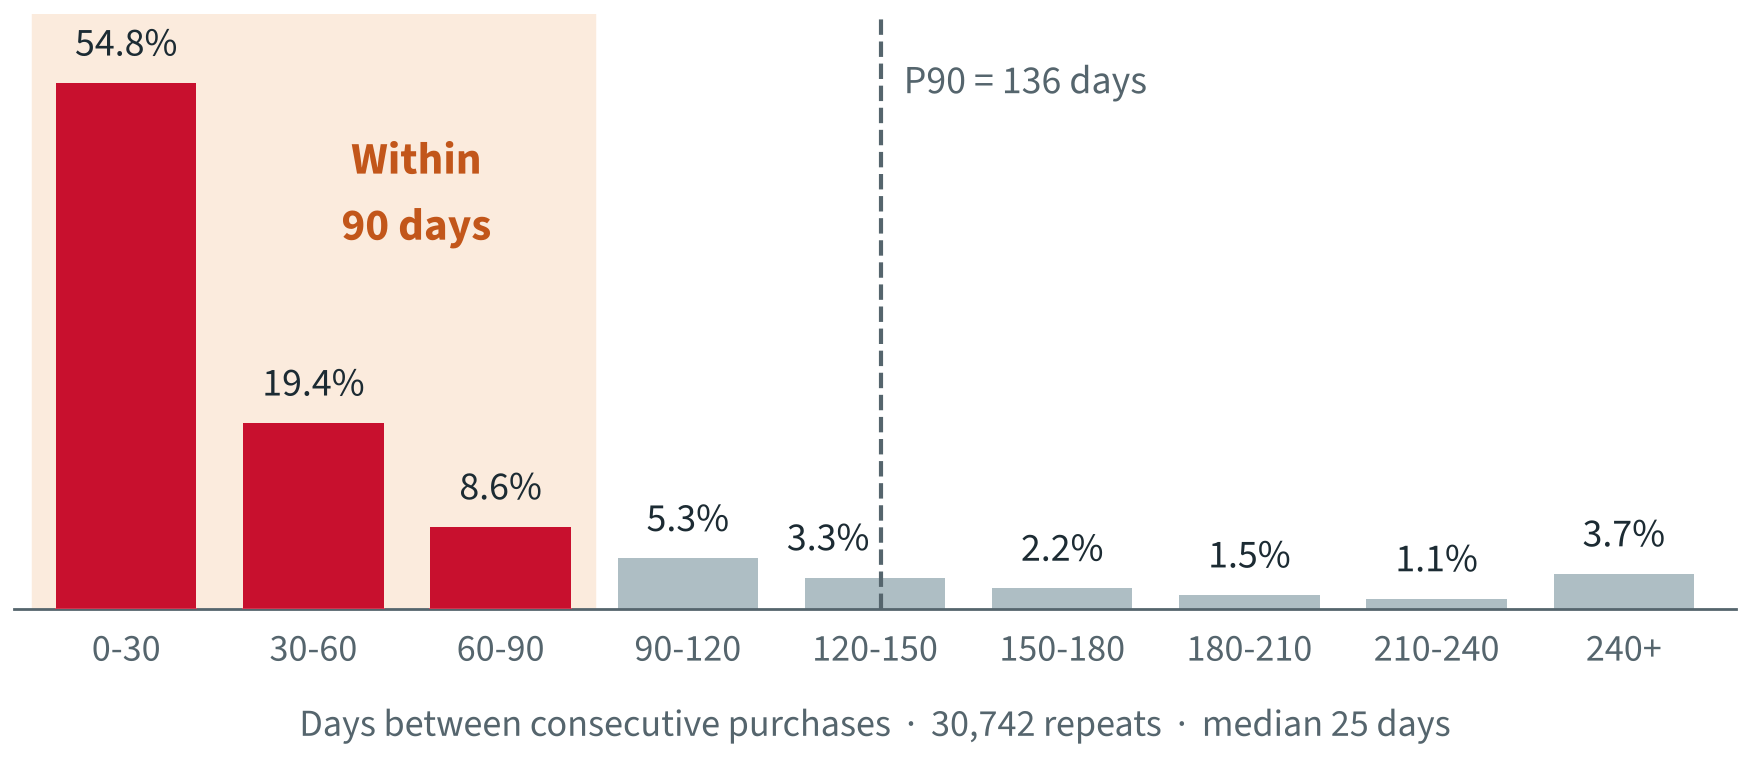
\includegraphics[width=\linewidth]{figures/repurchase_gap.png}
    \column{.52\textwidth}
    \small
    \setlength{\arrayrulewidth}{0.6pt}
    \renewcommand{\arraystretch}{1.15}
    \begin{tabular}{|>{\raggedright\arraybackslash}p{1.35cm}>{\raggedright\arraybackslash}p{2.75cm}>{\raggedright\arraybackslash}p{1.85cm}|}
      \hline
      \rowcolor{hustred}\textcolor{white}{\textbf{$H$}} & \textcolor{white}{\textbf{Repeat purchases within $H$}} & \textcolor{white}{\textbf{Training weeks left}}\\
      \rowcolor{cardgray}60 days & 74.2\% & 37\\
      \bfseries 90 days & \bfseries 82.8\% & \bfseries 24\\
      \rowcolor{cardgray}120 days & 88.1\% & 10\\
      \hline
    \end{tabular}\par
    \vspace{5pt}
    {\small\color{hustred}Short $H$ $\rightarrow$ many false churn labels. Long $H$ $\rightarrow$ late detection, less training data.\par}
  \end{columns}
  \vspace{2pt}
  \infocard{\dimexpr.333\textwidth-18pt\relax}{1.32cm}{%
    {\Large\bfseries\color{hustred}54.8\%}\\[2pt]
    {\scriptsize\color{inkgray}of repeat purchases within 30 days: the largest bin, but not enough}}\hfill
  \infocard{\dimexpr.333\textwidth-18pt\relax}{1.32cm}{%
    {\Large\bfseries\color{hustred}82.8\%}\\[2pt]
    {\scriptsize\color{inkgray}of repeat purchases within 90 days}}\hfill
  \infocard[hustred]{\dimexpr.333\textwidth-18pt\relax}{1.32cm}{\color{white}%
    {\large\bfseries $R_{\max}$ = 136 days (P90)}\\[2pt]
    {\scriptsize No purchase for 136+ days = already gone, nothing left to predict.}}
  % Speaker notes (Lam): We define churn as no purchase within $H$ days, and we set $H$ from
  % the purchase rhythm. More than half of repeat purchases happen within 30 days, but that
  % cutoff would miss too many. At 60 days, one in four repeat purchases would arrive after
  % we had already called the customer churned. At 120 days, we gain only five points but
  % training data drops from 24 weeks to 10. So 90 days is the balance: it covers 83\% of
  % returns. And anyone silent for more than 136 days is effectively gone. (About 35
  % seconds)
\end{frame}

\begin{frame}{Customer segments}{Six behaviour groups; two hold 63\% of revenue}
  \begin{columns}[T]
    \column{.45\textwidth}
    \small
    \renewcommand{\arraystretch}{1.5}
    \begin{tabular}{@{\hspace{6pt}}p{2.75cm}p{3.15cm}@{}}
      \rowcolor{hustred}\textcolor{white}{\textbf{Segment}} & \textcolor{white}{\textbf{Rule}}\\
      \rowcolor{black!20}\textcolor{hustred}{\textbf{Champions}} & Top 10\% M, R $\le$ 90\\
      \rowcolor{black!8}\textcolor{hustred}{\textbf{VIP at risk}} & Top 10\% M, R $>$ 90\\
      \rowcolor{black!20}Loyal & R $\le$ 90, F $\ge$ 4\\
      \rowcolor{black!8}Developing & R $\le$ 90, F = 2--3\\
      \rowcolor{black!20}One-time recent & R $\le$ 90, F = 1\\
      \rowcolor{black!8}Inactive & R $>$ 90
    \end{tabular}
    \column{.53\textwidth}
    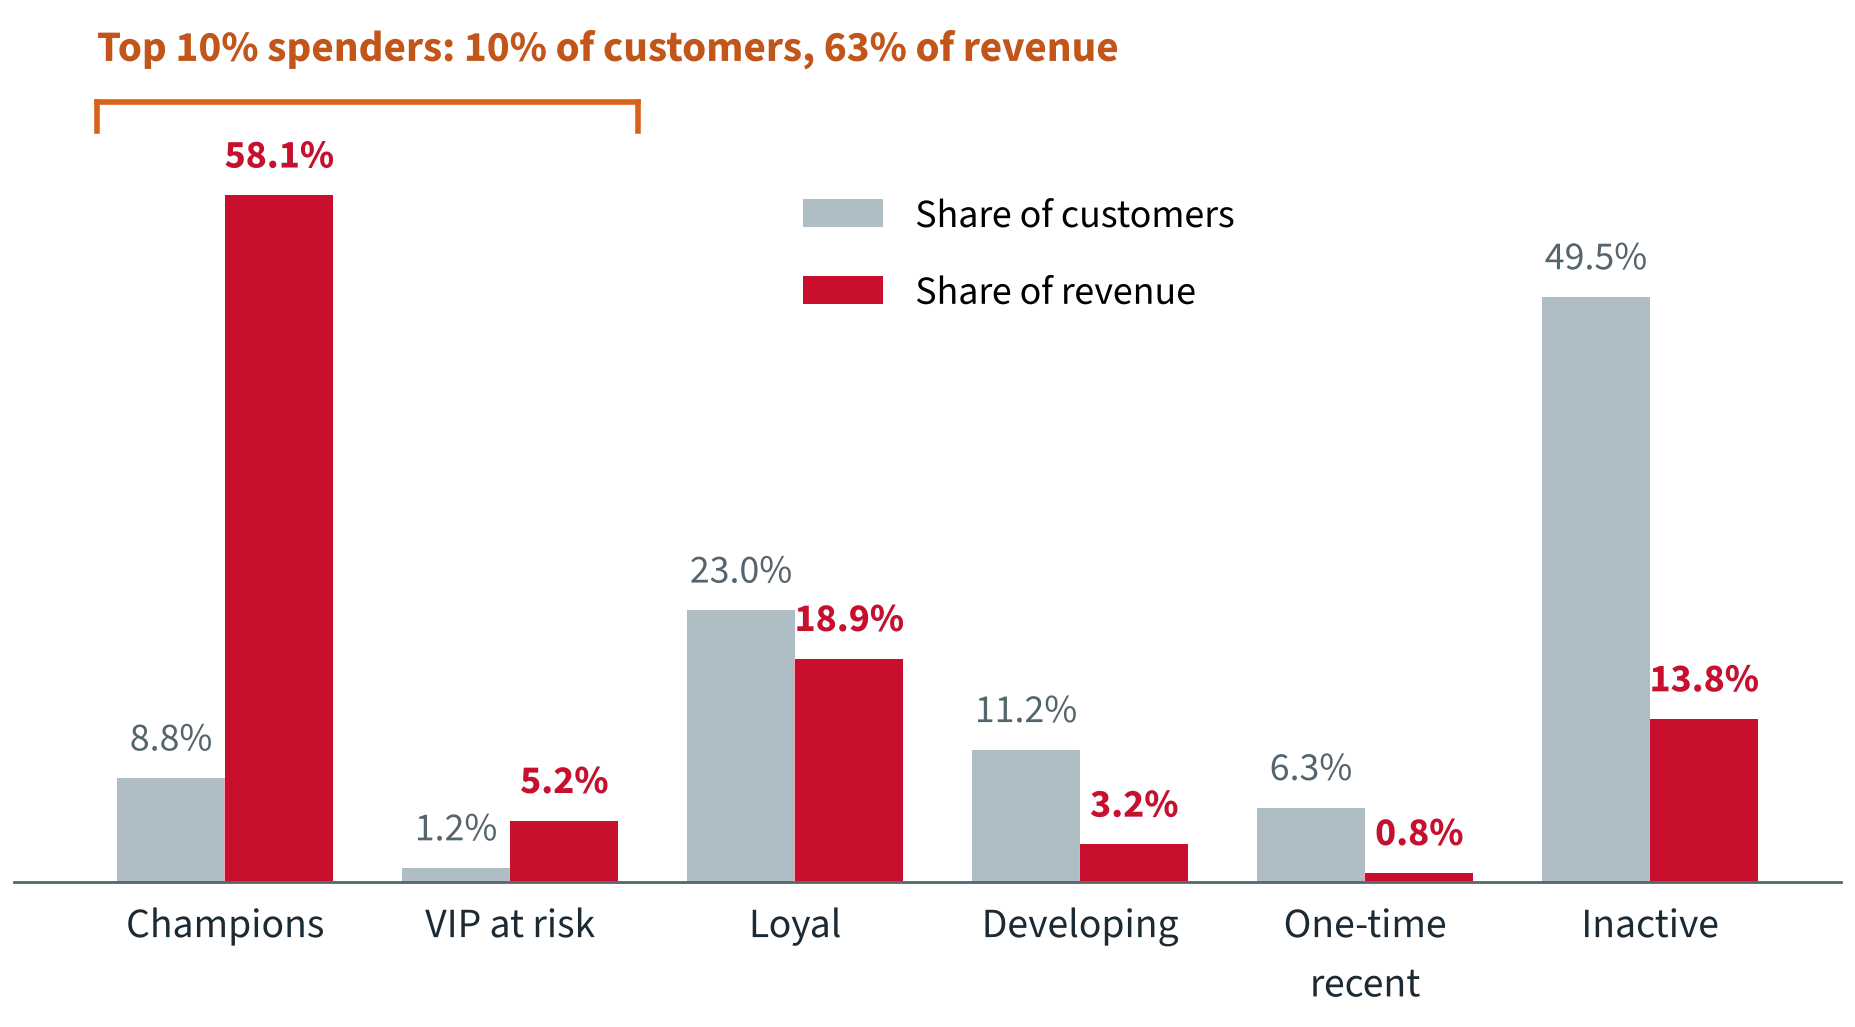
\includegraphics[width=\linewidth]{figures/rfm_segment_share.png}
  \end{columns}
  % Speaker notes (Lam): With that 90-day line and a spend threshold at the top 10\%, we
  % built our RFM segments: recency tells us who is still active, frequency how habitual
  % they are, and spend how valuable they are. The result is very concentrated: Champions
  % and VIP at risk are only 10\% of customers but bring 63\% of revenue. VIP at risk are
  % exactly the high-value customers who have crossed the 90-day line. Meanwhile half of all
  % customers are already inactive and bring only 14\%. So the next step is to predict which
  % valuable customers are about to cross that line, before they do. (About 35 seconds)
\end{frame}
